\chapter{Preliminaries}

\label{chapter:preliminaries}
\section{Homogenous coordinate system}

In projective geometry, the homogenous coordinate system is used in the same way as Cartesian coordinates are in Euclidean geometry.
To transform a point $x=(u, v)^T$ from cartesian coordinates to homogenous, simply append $1$ as the third coordinate: $x=(u, v, 1)^T$.
Homogenous coordinates are used to simplify the 2D transformation operations: 


\begin{equation}
    m_1 = 
    S R
    m_0
    + \vec{t}
\end{equation}
where 
$\begin{bmatrix} x_0 \\ y_0 \end{bmatrix}$
is an original point,
$\begin{bmatrix} x_1 \\ y_1 \end{bmatrix}$
is a transformed point,
$S = \begin{bmatrix} s_x & 0 \\ 0 & s_y \end{bmatrix}$ 
is a scale matrix, 
$R = \begin{bmatrix} cos(\theta) & -sin(\theta) \\ sin(\theta) & cos(\theta) \end{bmatrix}$ 
is a rotationa matrix and 
$\vec{t} = \begin{bmatrix} t_x \\ t_y \end{bmatrix}$ 
is a translation vector.

To apply a transformation, it is required to make a sequence of matrix multiplications, but this is not the case with translation - an addition operation is needed for that. 
Here are these operation in projective geometry:

\begin{equation}
    \begin{bmatrix} m_1 \\ 1 \end{bmatrix} = 
    S_H R_H T_H
    \begin{bmatrix} m_0 \\ 1 \end{bmatrix}    
\end{equation}
where 
$S_H = \begin{bmatrix} s_x & 0 & 1\\ 0 & s_y & 1 \\ 0 & 0 & 1\end{bmatrix}$
, 
$R_H = \begin{bmatrix} cos(\theta) & -sin(\theta) & 0 \\ sin(\theta) & cos(\theta) & 0 \\ 0 & 0 & 1 \end{bmatrix}$
and
$T_H = \begin{bmatrix} 1 & 0 & t_x\\ 0 & 1 & t_y \\ 0 & 0 & 1 \end{bmatrix}$
is a translation matrix.

So in the homogenous coordinate system, all 2d transformations can be combined and expressed as matrix multiplications.

\subsection{Infinity}
\begin{figure}[h]
    \centering
    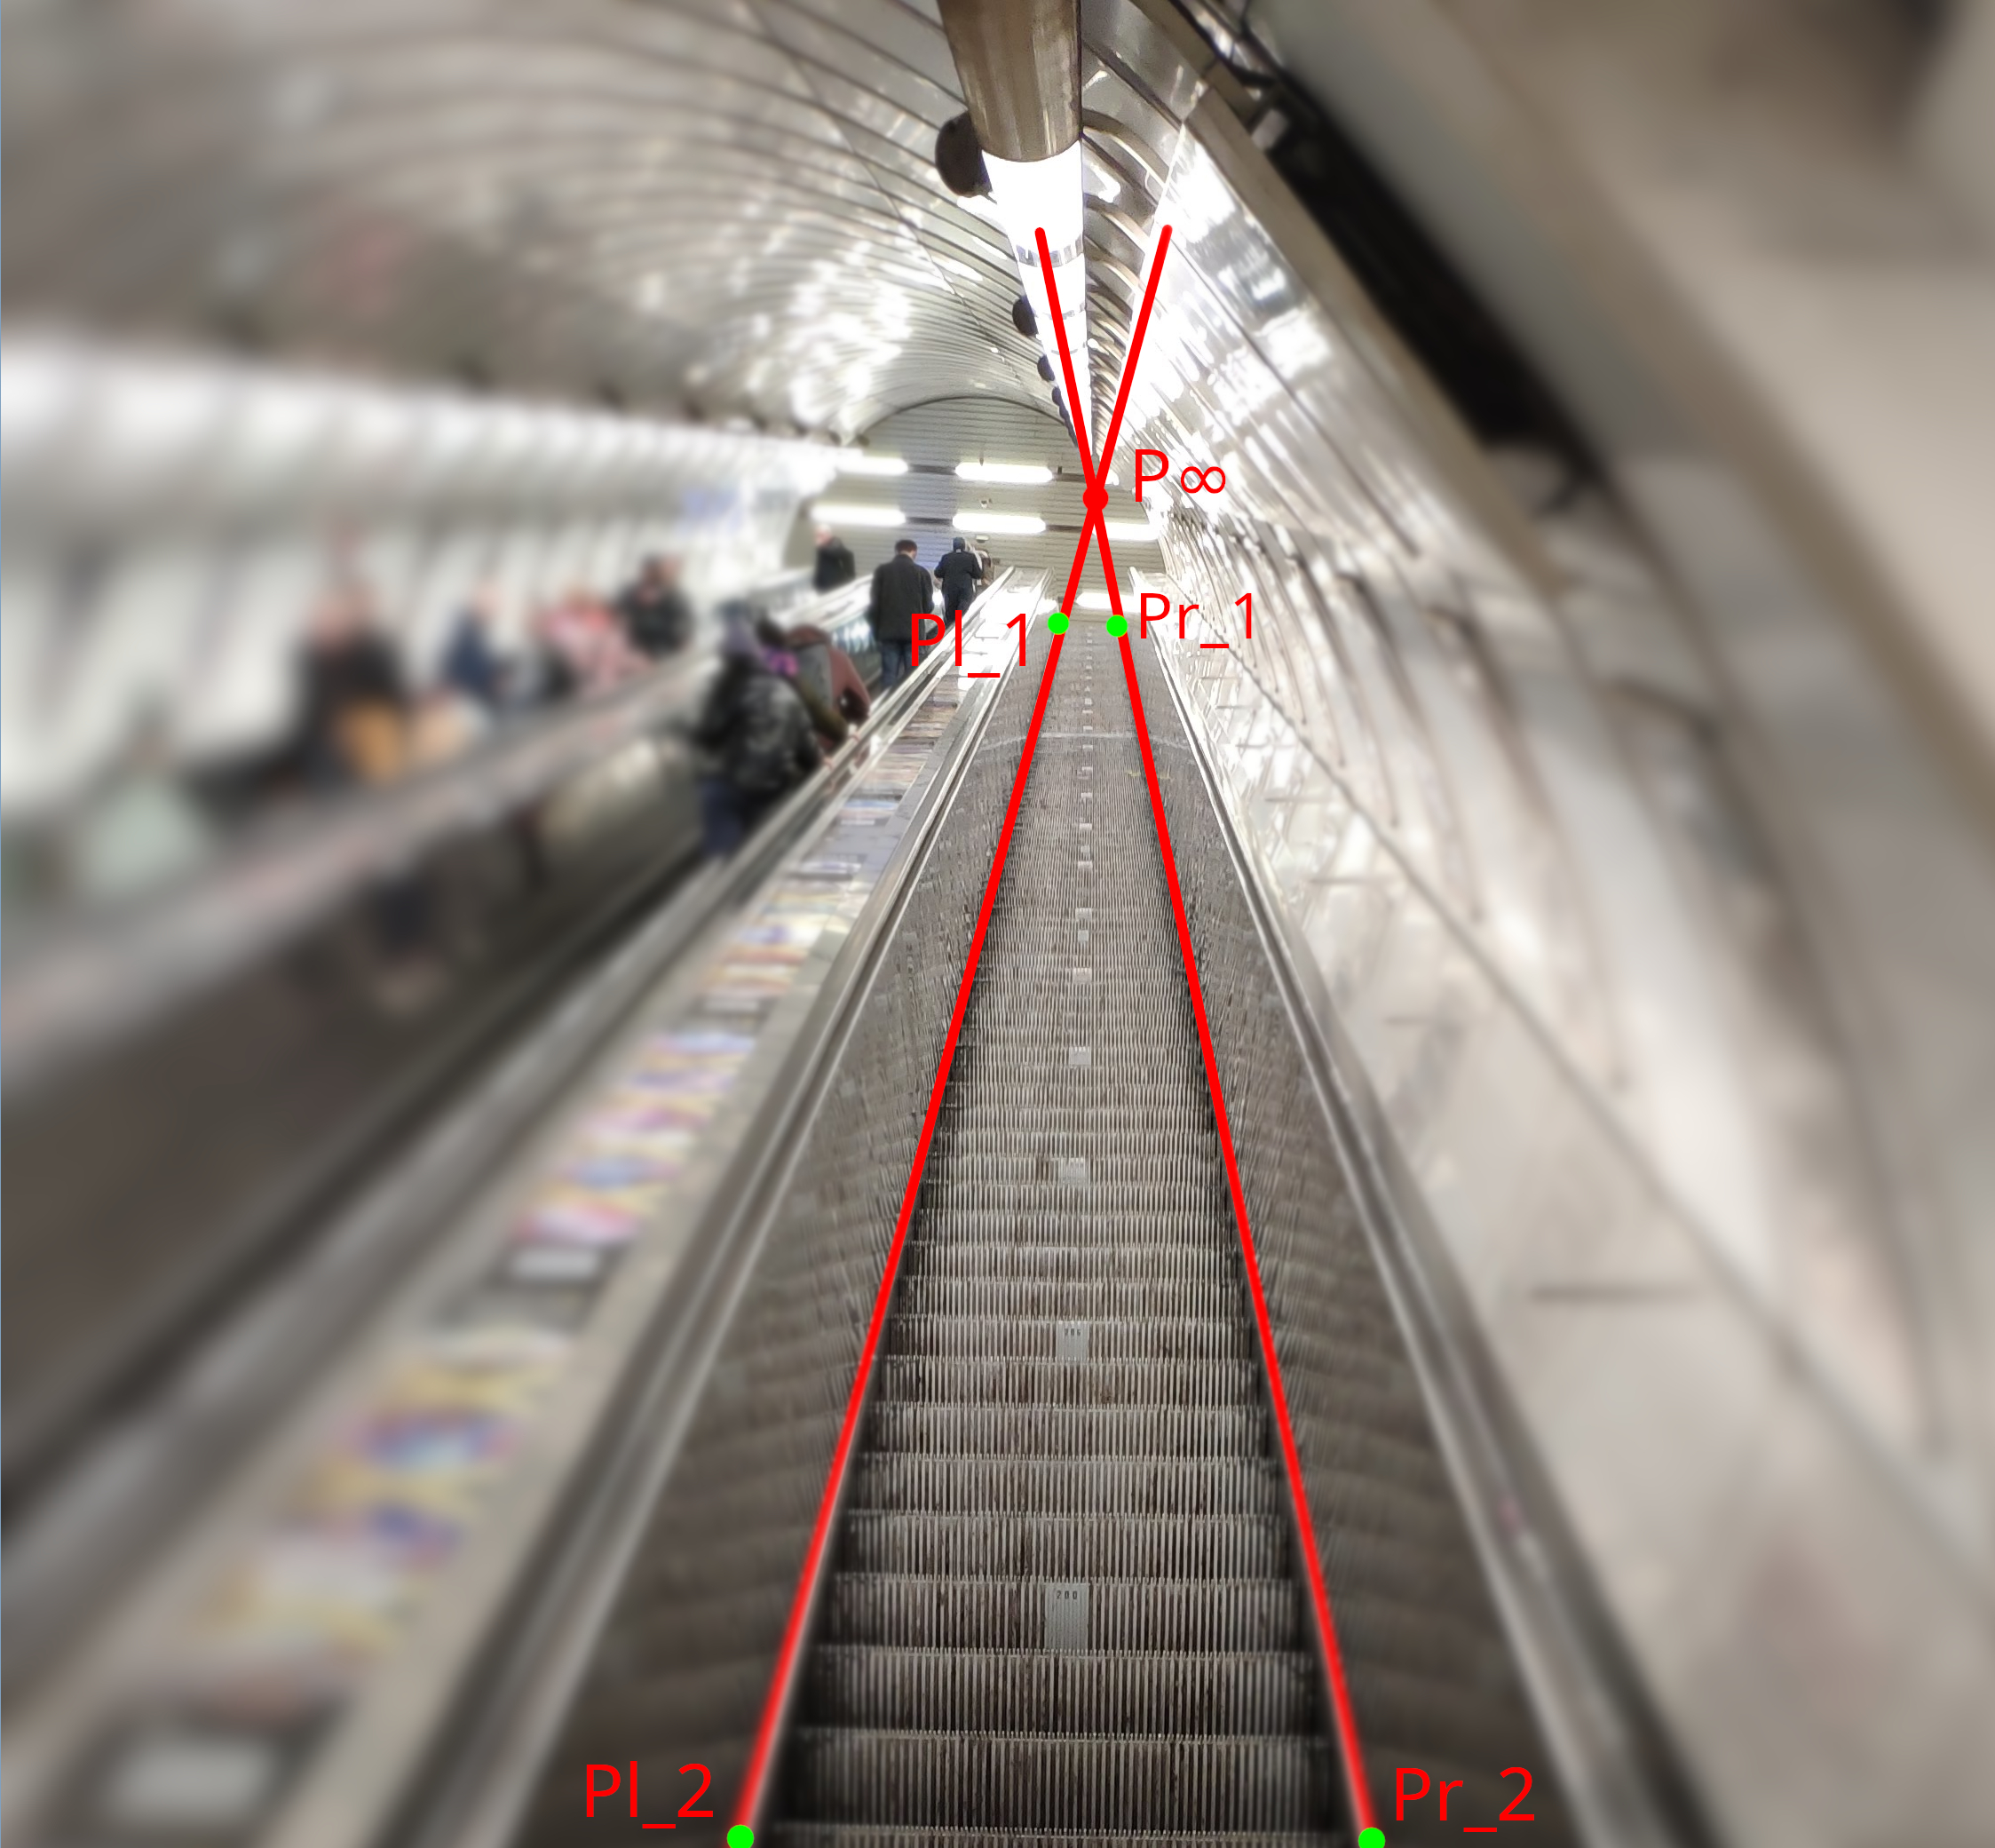
\includegraphics[width=0.7\textwidth]{graphics/parallel_intersection.jpg}
    \caption{Parallel lines intersection}
    \label{fig:intersection_parallel}
\end{figure}

\begin{figure}[h]
    \centering
    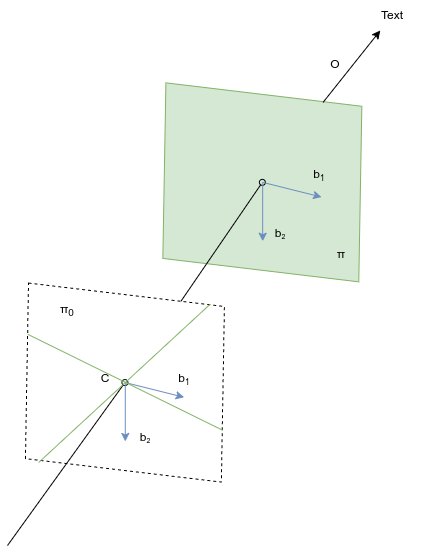
\includegraphics[width=.5\textwidth]{graphics/homogenous.png}
    \caption{Scheme of homogenous coordinates}
    \label{fig:homogenous}
\end{figure}

In Euclidian geometry, parallel lines are the lines that have no intersection point. 
In projective geometry, parallel lines intersect at a point $x$ at infinity. 
How is it possible? 
In the image \autoref{fig:intersection_parallel} let $l_r = Pr_1 \cap Pr_2 $ and $l_l = Pl_1 \cap Pl_2$. 
In the 3D world, we know that lines $l_l \parallel l_r$, but after projection on the image plane $\Pi$, we can calculate - in this case even see - the intersecting point $P_{\infty}$. 

Both line and point in a homogenous coordinates can be expressed as vector of three numbers: a homogenous point $x = (x, y, z)^T$ will be $m = (\frac{x}{z}, \frac{y}{z})^T$, line $l = (a, b, c)^T$, where $a, b, c$ are parameters of a line equation $ax + by + c = 0$. 
In general case point at infinity is called an \textit{ideal point} and it is not seen on the image, it's coordinates can be expressed as $x_{\infty} = (u, v, 0)^T, \{u, v\} \neq 0$. Same about line - such line is called \textit{ideal line} and it's coordinates are $l = (0, 0, c)^T, c \neq 0$. In algebraic representation, both ideal point and line are lying at the plane $\Pi_0$ (\autoref{fig:homogenous}, green lines).

\subsection{Vanishing points}
% TODO!

\section{Pinhole camera model}
A pinhole camera - or a canonical perspective camera model - is a model of a simple camera without optics.
The first example is a camera obscura - a dark room with a small hole through which the image from outside is projected on the opposite wall. 
This model can be used to express camera geometry with a field of view angles less than $180^{\circ}$.

\subsection{Camera coordinate system}
\begin{figure}[h]
    \centering
    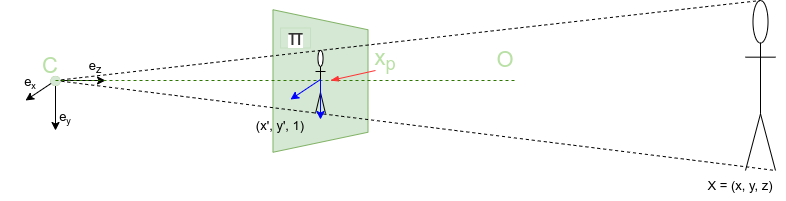
\includegraphics[width=1\textwidth]{graphics/td_scene.png}
    \caption{The pinhole camera model working scheme}
    \label{fig:td_scene_3d}
\end{figure}

\begin{figure}[h]
    \centering
    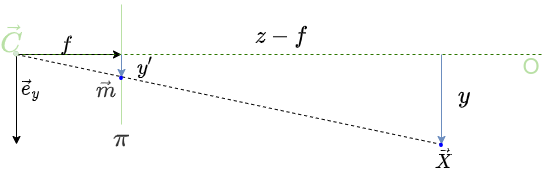
\includegraphics[width=0.9\textwidth]{graphics/td_scene_yz.png}
    \caption{The pinhole camera model, y-z plane}
    \label{fig:td_scene_yz}
\end{figure}

\begin{figure}[h]
    \centering
    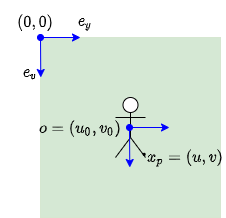
\includegraphics[width=.4\textwidth]{graphics/td_scene_xy.png}
    \caption{The pinhole camera model, x-y plane}
    \label{fig:td_scene_xy}
\end{figure}

In the physical implementation of the Obscure camera, the projective plane is on the opposite side from the Projection centre (or Camera centre $C$ in the pinhole camera model), the image is reversed and mirrored, but in most computer vision literature, authors assume that it is on the same side as an object (see \autoref{fig:td_scene_3d}).
In \autoref{fig:td_scene_3d} we are looking through a camera with camera center $C$ in a coordinate system with origin at $C$ and basis vectors $(e_x, e_y, e_z)$ on a human. 
Each point $X = (x, y, z)^T$ in a world coordinate system has it's projection $x_p = (u, v)^T$ on a plane $\Pi$ which is located on a distance 1 from a camera center (\autoref{fig:td_scene_yz}). 
Optical axis $O$ is a ray perpendicular to plane $\Pi$, and on the image the point $ O \cap \Pi = o$ is a center of the image, see \autoref{fig:td_scene_xy}).

\subsection{Camera calibration matrix}
\begin{figure}[h]
    \centering
    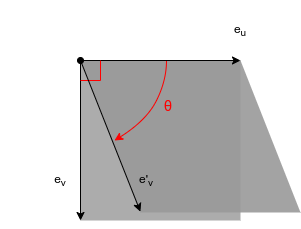
\includegraphics[width=.6\textwidth]{graphics/pixel.png}
    \caption{Scheme of pixel, changing the image (inner) reference frame}
    \label{fig:Kframes}
\end{figure}
Camera calibration matrix - a matrix that includes camera \textit{intrinsic} parameters - pixel size ($e_u$ and $e_v$) and pixel skew angle ($\theta$), as on \autoref{fig:Kframes}, pixel aspect ratio $\bf{a}$ and principle point coordinates $o = (u_0, v_0)$ \autoref{fig:td_scene_xy}.
\begin{equation}
    \textrm{K =}\begin{bmatrix}
        af & -a f cot(\theta) & u_0 \\
        0 & f / sin(\theta) & v_0 \\
        0 & 0 & 1 \\
    \end{bmatrix} 
    \textrm{ units: } [f]=px, [u_0]=px, [v_0]=px, [a]=1
\end{equation}


Where $f$ is a focal length used to convert world length ratios to pixels.

In the modern world, every digital camera has a calibration matrix with a square pixel, so in most cases, the camera matrix looks like this:

\begin{equation}
    \label{eq:kmat}
    \textrm{K = }\begin{bmatrix}
        f_x & 0 & u_0 \\
        0 & f_y & v_0 \\
        0 & 0 & 1 \\
    \end{bmatrix}    
\end{equation}

\subsection{Projection matrix}

\begin{figure}[h]
    \centering
    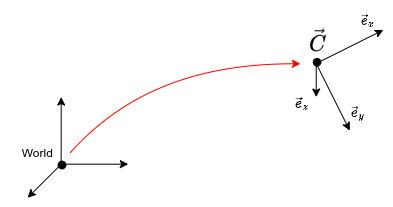
\includegraphics[width=.5\textwidth]{graphics/frames.png}
    \caption{Changing the world (outer) reference frame}
    \label{fig:frames}
\end{figure}

To translate a point from a world coordinate frame to an image coordinate frame, the Image projection matrix $P$ is used. 
The canonical projection matrix $P_0$ assumes that the camera is in the world coordinate centre and that the calibration matrix $K = I$
\begin{equation}
P_0 = \begin{bmatrix} I & | & \vec{0} \end{bmatrix} = 
    \begin{bmatrix}
    1 & 0 & 0 & 0 \\
    0 & 1 & 0 & 0 \\
    0 & 0 & 1 & 0 \\
    \end{bmatrix}    
\end{equation}

However, this case is degenerate. 
As far as each camera is different, the canonical projection matrix is never used. Instead, image projection matrix $P$ is used, with applied calibration matrix $K$ to transform canonical $P_0$ to perspective $P$:

\begin{equation}
P = K \begin{bmatrix} I & | & \vec{0} \end{bmatrix} = 
    \begin{bmatrix} 
    f_x & 0 & u_0 & 0 \\
    0 & f_y & v_0 & 0 \\ 
    0 & 0 & 1 & 0 \\
    \end{bmatrix}    
\end{equation}

However, usually the world coordinate centre is not located at point $\vec{C}$ \autoref{fig:frames}. 
Usually it is rotated using a rotation matrix $R$ and translated on vector $\vec{t}$ where $R$ is a $3x3$ matrix with $det(R) = 1$ and $R^{-1} = R^T$. 
So, in the general case:
\begin{equation}
    P = K \begin{bmatrix} R & | & \vec{t} \end{bmatrix} = 
    K \begin{bmatrix} R & | & - R \bf{C} \end{bmatrix}
\end{equation}

where $\vec{C}$ is often used as a camera position in a world reference frame. 
So matrix $\bf{P}$ have six intrinsic parameters: three Euler angles and three translation components. 

\subsection{Projection equation}

Image point $m = (u, v)^T$ can be obtained from a 3D point $X$ using matrix $\bf{P}$:

\begin{equation}
    \label{eq:projection}
    \lambda \begin{bmatrix} 
        u \\ v \\ 1 \end{bmatrix} = P \begin{bmatrix} x \\ y \\ z \\ 1
    \end{bmatrix}
\end{equation}

\begin{equation}
    \lambda \begin{bmatrix} 
    \vec{m} \\ 1 \end{bmatrix} = P \begin{bmatrix} \vec{X} \\ 1
        \end{bmatrix}
\end{equation}
Where $\lambda \neq 0$

\section{Epipolar geometry}

\subsection{Skew-symmetric 3x3 matrix}
As it is written in a book \cite{hartley_zisserman_2004}, p. 581, a skew-symmetric or antisymetric matrix is such matrix $[b]_{\times}$ that $[b]_{\times}^T = -[b]_{\times}$. 
For vector $b = (b_1, b_2, b_3)^T$:
\begin{equation}
    [b]_{\times} = \begin{bmatrix}
        0 & -b_3 & b_2 \\ 
        b_3 & 0 & b_1 \\ 
        -b_2 & b_1 & 0 \\ 
    \end{bmatrix}    
\end{equation}

This matrix has some essential properties, but the most important in this thesis - it generalizes across a product as matrix multiplication.
\begin{equation}
    a \times b = [a]_{\times} b
\end{equation}

\subsection{Epipolar geometry}
\begin{figure}[h]
    \centering
    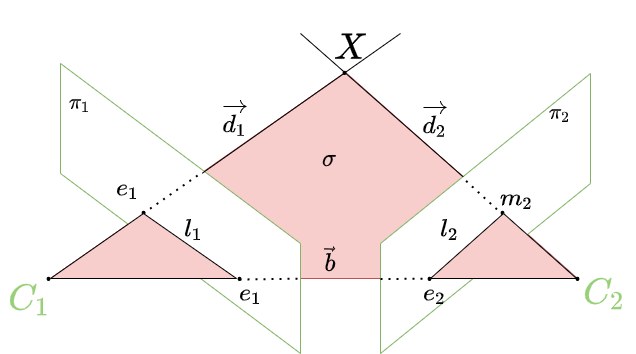
\includegraphics[width=1\textwidth]{graphics/epipolar.png}
    \caption{Epipolar geometry scheme}
    \label{fig:epipolar_std}
\end{figure}

\autoref{fig:epipolar_std} shows a scheme of two cameras with different camera centers $C_1$ and $C_2$ connected with a base line $\vec{b} = C_2 - C_1$. 
Both of them are seen as some 3d point $X$. 
This point projections are $m_1$ and $m_2$ respectivly. 
Points $C_1, C_2$ and $X$ form an \textit{epipolar plane} $\sigma$.
$\sigma \cap \pi_1 = l_1$ and $\sigma \cap \pi_2 = l_2$ are images of \textit{epipolar lines}. 
Epipolar line $l_1$ passes through \textit{epipole} $e_1$, where $\lambda [e_1 | 1]^T = \bf{P_2} C_1$, same with $\lambda [e_2 | 1]^T = \bf{P_1} C_2$.

\subsection{Epipolar constraint}

Having a set of two cameras the relationship between them and constraints on them can be expressed by two new matrices \textit{Essential matrix} $E \in \mathbb{R}^{3x3}, rank(E) = 2$, \autoref{eq:E} and \textit{Fundamental matrix} $F \in \mathbb{R}^{3x3}, rank(F) = 2$, \autoref{eq:F}
\begin{equation}
    \label{eq:E}
    E = R_2 [C_2 - C_1]_{\times} R_1^T = [-\vec{t}_{21}]_{\times}R_{21} = [\vec{b}]_{\times} R_{21}
\end{equation}
\begin{equation}
    \label{eq:F}
    F = K_2^{-T} R_2 [C_2 - C_1]_{\times} R_1^T K_1^{-1} = K_2^{-T} [-\vec{t}_{21}]_{\times} R_{21} K_1^{-1} = K_2^{-T} E K_1^{-1}
\end{equation}
where 
$R_{21} = R_2 R_1^T$ is a relative camera rotation and 
$\vec{t}_{21} = -R_2 \vec{b} = \vec{t}_2 - R_{21}\vec{t}_1$ is a relative camera translation.
The matrix $E$ can be calculated from image correspondences, but the translation scale $b$ is lost since E is homogenous, so after a decomposition of $E$ to $R$ and $b$ the translation distance will be lost.

An algebraic expression of important properties of matrix $F$:
\begin{equation}
    \label{eq:Fm2}
    \lambda l_1 = F^T \begin{bmatrix} m_2 \\ 1 \end{bmatrix}    
\end{equation}
\begin{equation}
    \label{eq:Fm1}
    \lambda l_2 = F \begin{bmatrix} m_1 \\ 1 \end{bmatrix}    
\end{equation}
\begin{equation}
    \label{eq:fefe}
    F \begin{bmatrix} e_1 \\ 1 \end{bmatrix} = F^T \begin{bmatrix} e_2 \\ 1 \end{bmatrix} = 0    
\end{equation}
\begin{equation}
    \label{eq:epiconstr}
    \begin{bmatrix} m_2 & | & 1 \end{bmatrix} F \begin{bmatrix} m_1 \\ 1 \end{bmatrix} = 0    
\end{equation}
Matrix $F$ maps points from $\pi_1$ to epipolar lines on $\pi_2$ and vice versa (\autoref{eq:Fm1} and \autoref{eq:Fm2}); epipoles $e_1$ and $e_2$ are right and left nullspaces basis vectors of $F$ respectivly (\autoref{eq:fefe}).
Epipolar constraint \autoref{eq:epiconstr} means that a point and it's corespondent line are on a same plane (\autoref{fig:epipolar_std}, plane $\sigma$).

\section{Stereovision}

\begin{figure}[h]
    \centering
    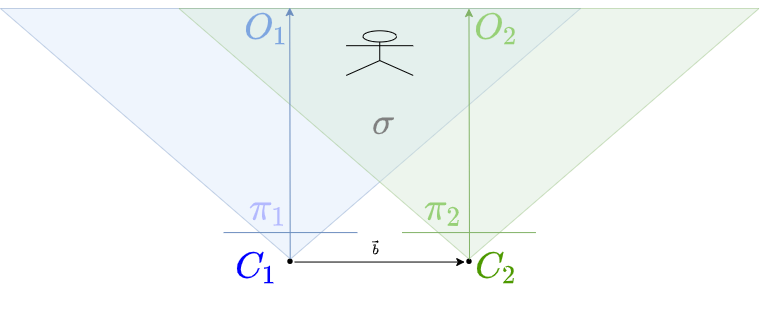
\includegraphics[width=1\textwidth]{graphics/stereopair.png}
    \caption{Scheme of stereovision}
    \label{fig:sch_stereo}
\end{figure}
\begin{figure}[h]
    \centering
    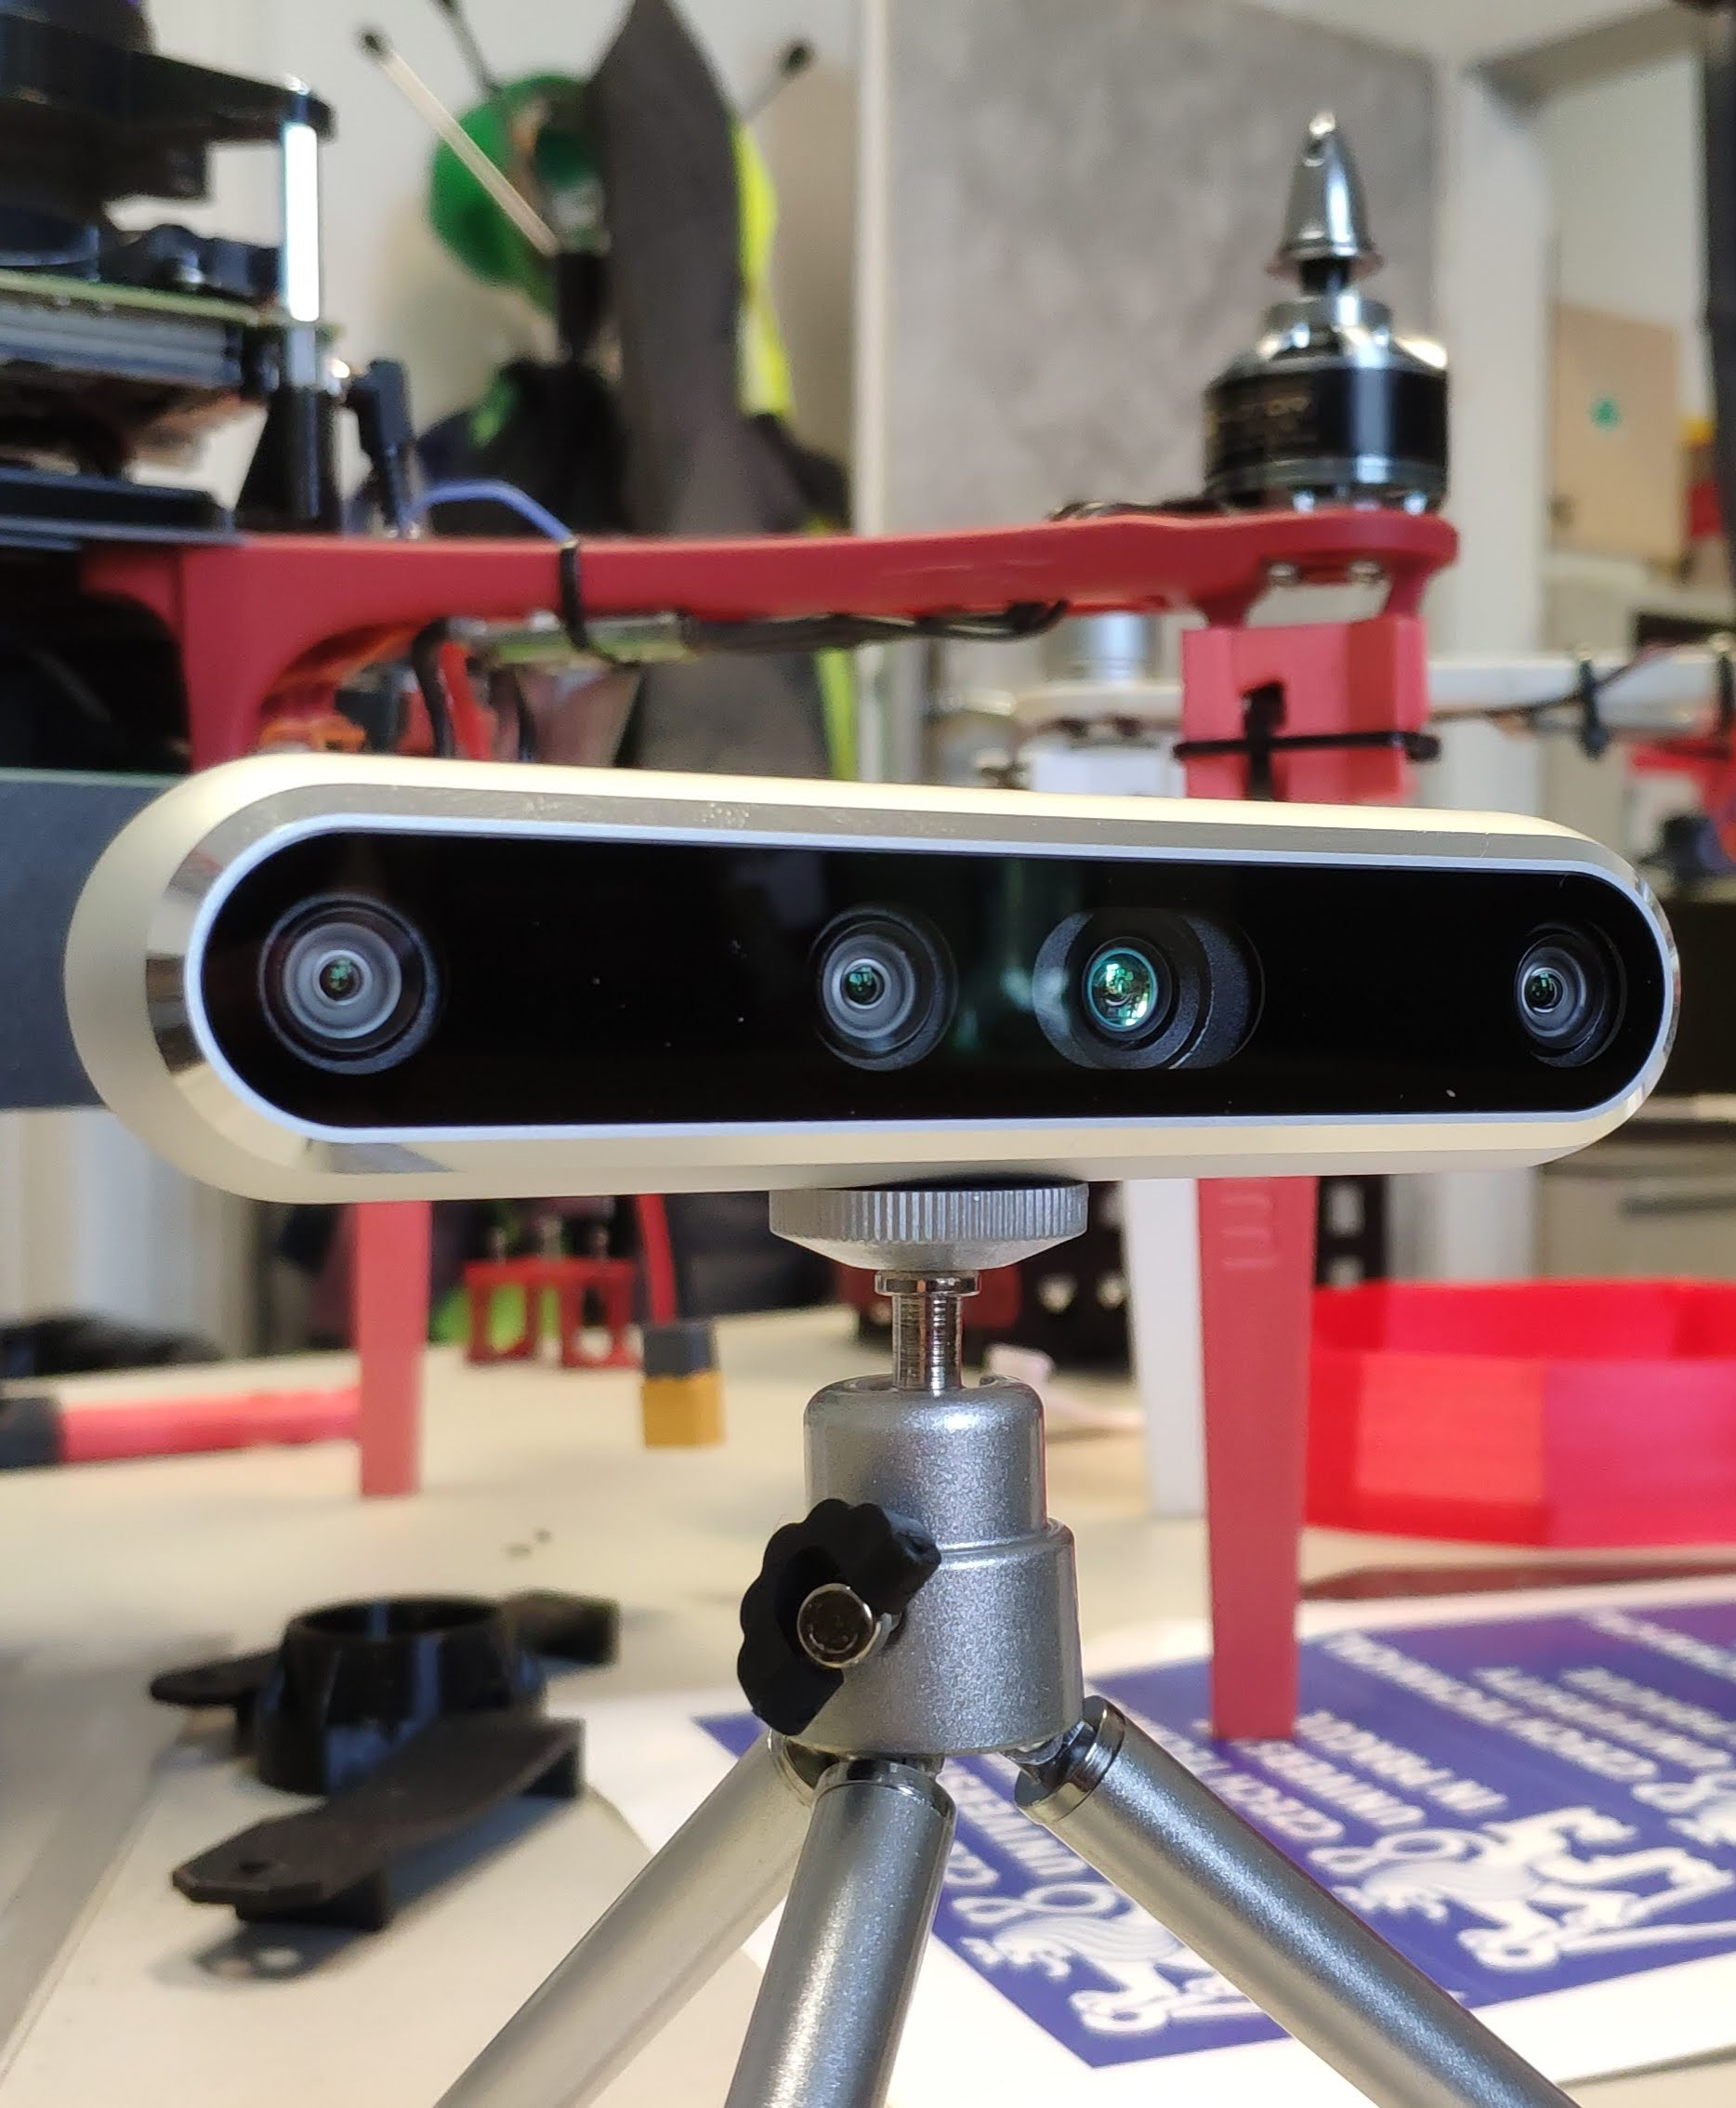
\includegraphics[width=0.5\textwidth]{graphics/stereo_example.jpg}
    \caption{Insustrial stereocamera example, Intel realsense D455}
    \label{fig:stereo_ex}
\end{figure}

\begin{figure}[h]
    \begin{subfigure}[b]{0.31\textwidth}
      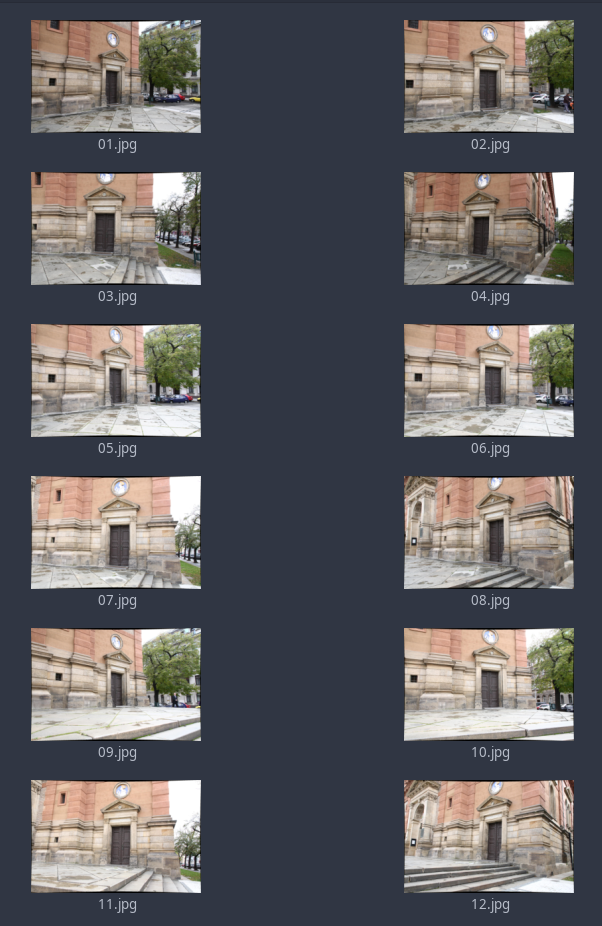
\includegraphics[width=\textwidth]{graphics/input_set.png}
      \caption{Input set of images.}
      \label{fig:pc_input}
    \end{subfigure}
    \hfill
    \begin{subfigure}[b]{0.65\textwidth}
      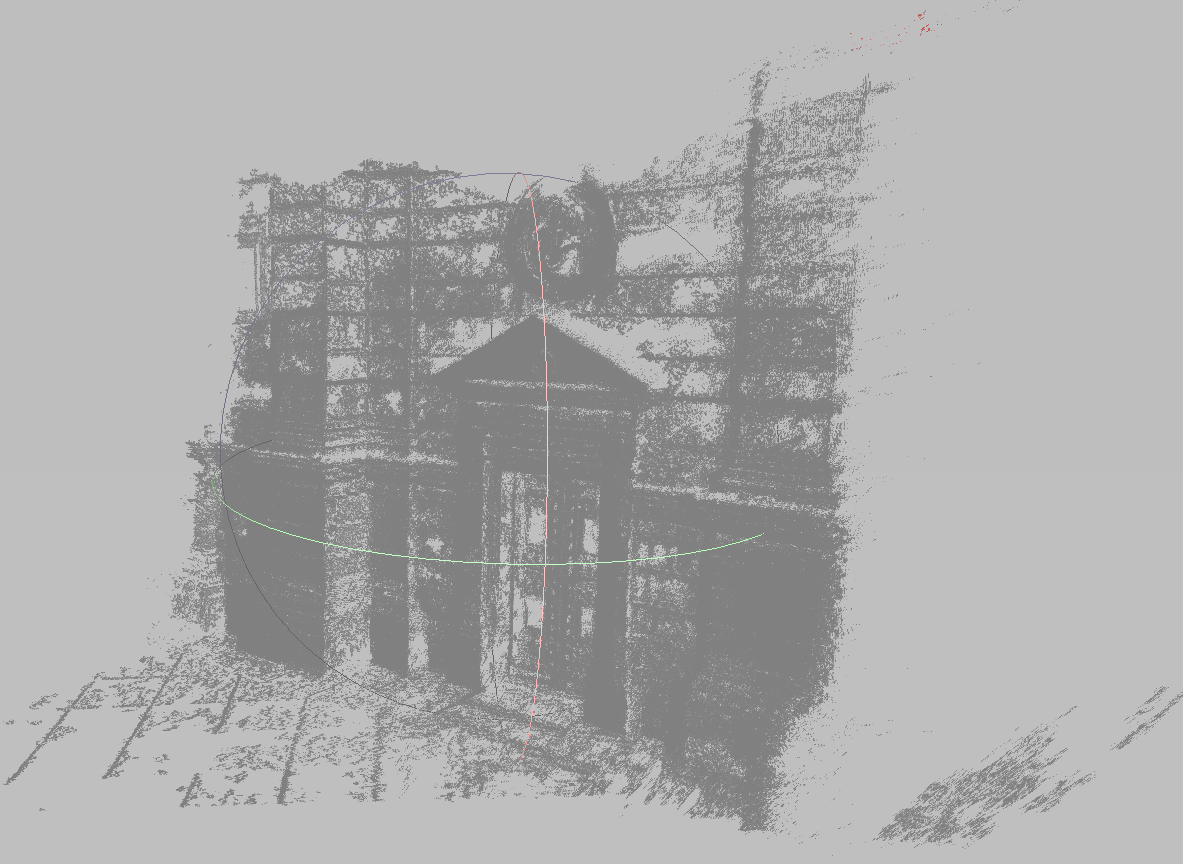
\includegraphics[width=\textwidth]{graphics/reconstructed.png}
      \caption{reconstructed pointcloud.}
      \label{fig:pc_output}
    \end{subfigure}
    \caption{Three dimensional reconstruction from multiple cameras.}
    \label{fig:pc_recons}
\end{figure}

Computer stereovision is a process of extracting a stereo (depth) image from planar image or set of images of the same scene. Usually stereocamera has two simple cameras located on some distance $\vec{b}$ pointing to the same direction, same as human eye (the scheme \autoref{fig:sch_stereo} and an example of a stereocamera \autoref{fig:stereo_ex}). 
Sometimes fusion of multiple cameras and other sensors can be used:
Intel Realsense \autoref{fig:stereo_ex} has two cameras, IR sensor in case if the images have almost no texture and a color sensor). 

\begin{equation}
    \label{eq:e1e2}
    e_1 = e_2 = \lambda \begin{bmatrix} 1 \\ 0 \\ 0 \end{bmatrix}
\end{equation}
\begin{equation}
    \label{eq:e1m1}
    \lambda l_1 = e_1 \times m1 = [e_1]_\times \begin{bmatrix} m_1 \\ 1\end{bmatrix}
\end{equation}
\begin{equation}
    \label{eq:F_simple}
    F = \lambda [e_1]_\times = \lambda \begin{bmatrix}
        0 & 0 & 0 \\
        0 & 0 & -1 \\
        0 & 1 & 0 \\
    \end{bmatrix}
\end{equation}

It is possible to calculate only non-zero multiple of $E$ from image correspondences, so the scene can be reconstructed only up to a scale, but knowing the thanslation vector $\vec{b}$ (\autoref{fig:sch_stereo}), means having a calibrated stereopair, all distances can be calculated in world coordinates frame.
By removing a rotation between cameras ($R = I$), all computations are simplified.

Corresponding epipolar lines lie on same image rows ($l_1 = l_2$), and intersects at "points at infinity" (\autoref{eq:e1e2}). 
Epipole is a point of intersecting all epipolar lines, so having the intersecting point ($e_1$) and image point epipolar line can be calculated (\autoref{eq:e1m1}), therefore considering \autoref{eq:Fm1}, \autoref{eq:e1e2} and \autoref{eq:e1m1} the \autoref{eq:F_simple} is true.

What is more, consider two correspondences $c_1 = (u_1, v)$ and $c_2 = (u_2, v) $. For a correspondences matcher it is more efficient to have a predefined corelation between features - and knowing the fact that $v$ coordinate is the same (up to some error) is good enough constraint that can accelerate matching (and looking for more features).

Using this approach it is possible to receive even a dense pointcloud as on \autoref{fig:pc_output}.


\section{Calibration}
\subsection{Single camera calibration}

\begin{figure}[h]
    \centering
    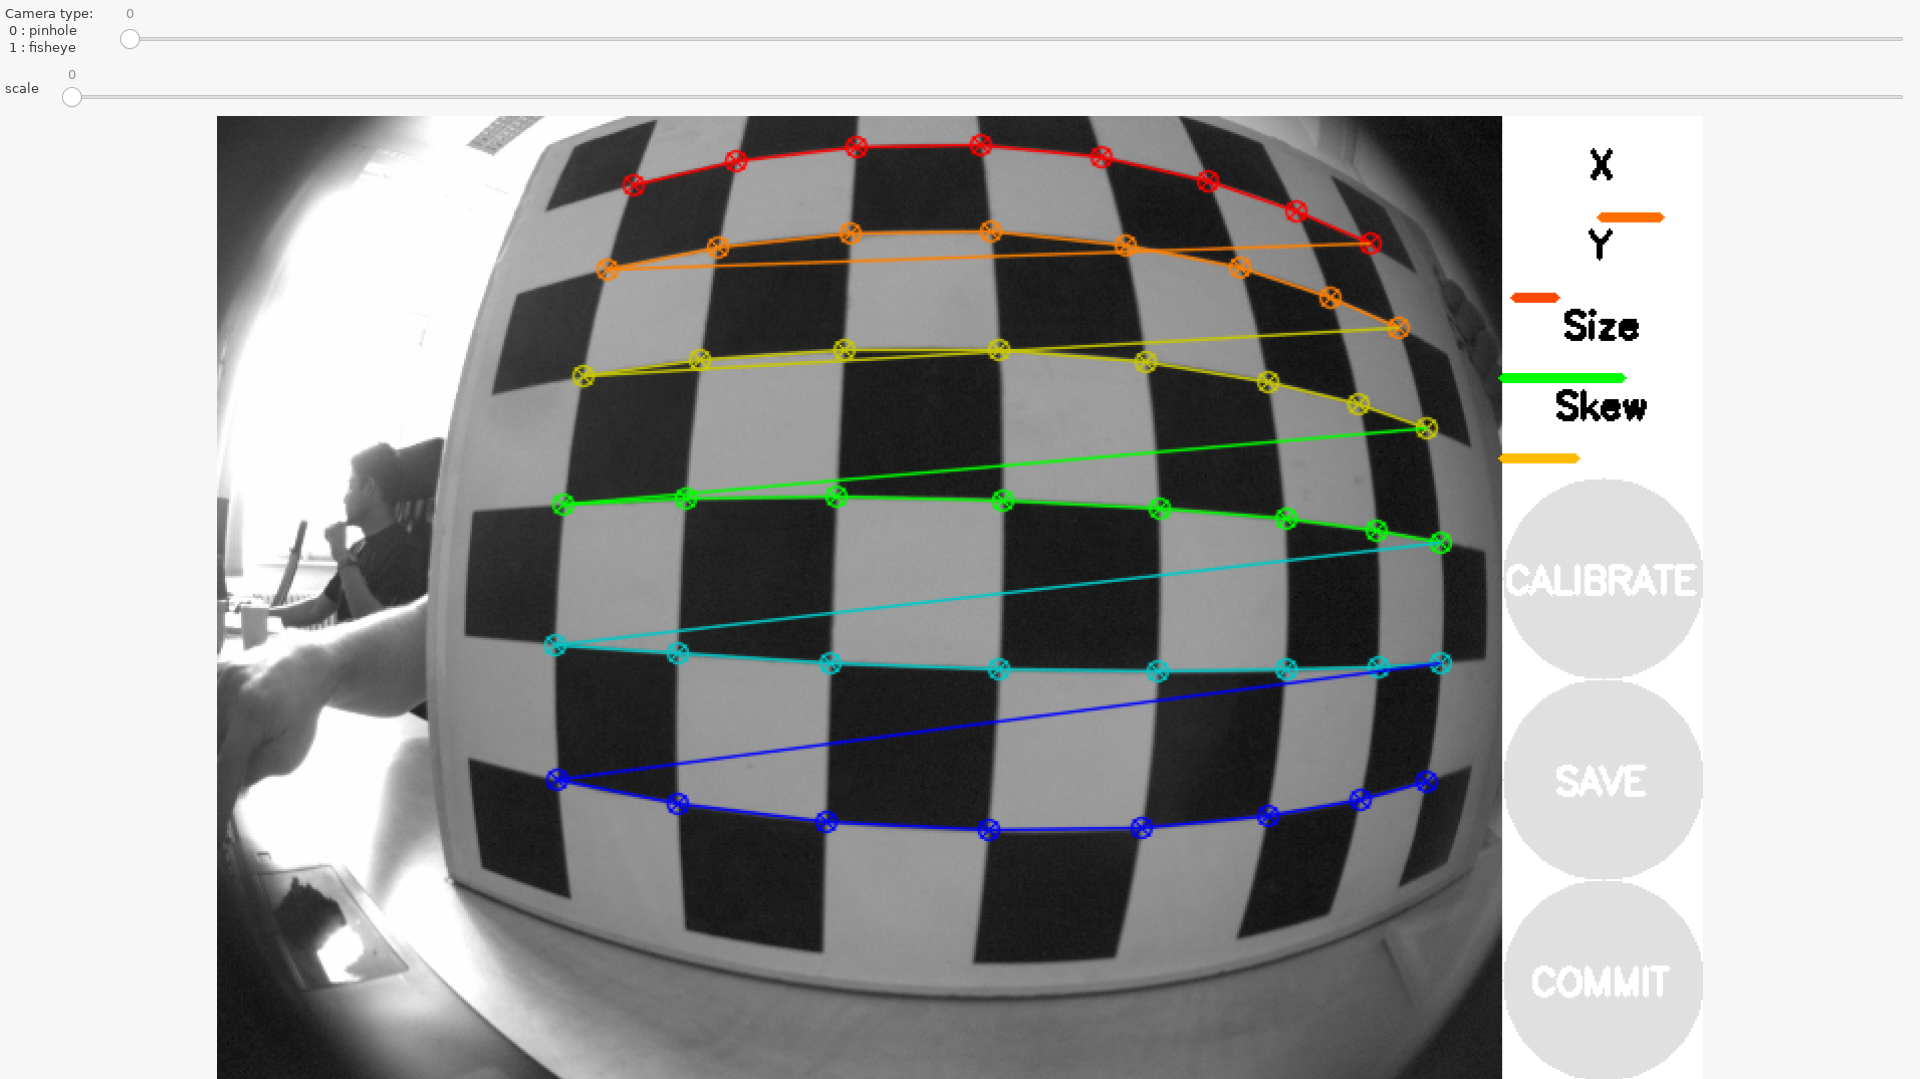
\includegraphics[width=.6\textwidth]{graphics/calibration.png}
    \caption{Calibration process}
    \label{fig:calib}
\end{figure}

\begin{figure}[h]
    \begin{subfigure}[b]{0.45\textwidth}
      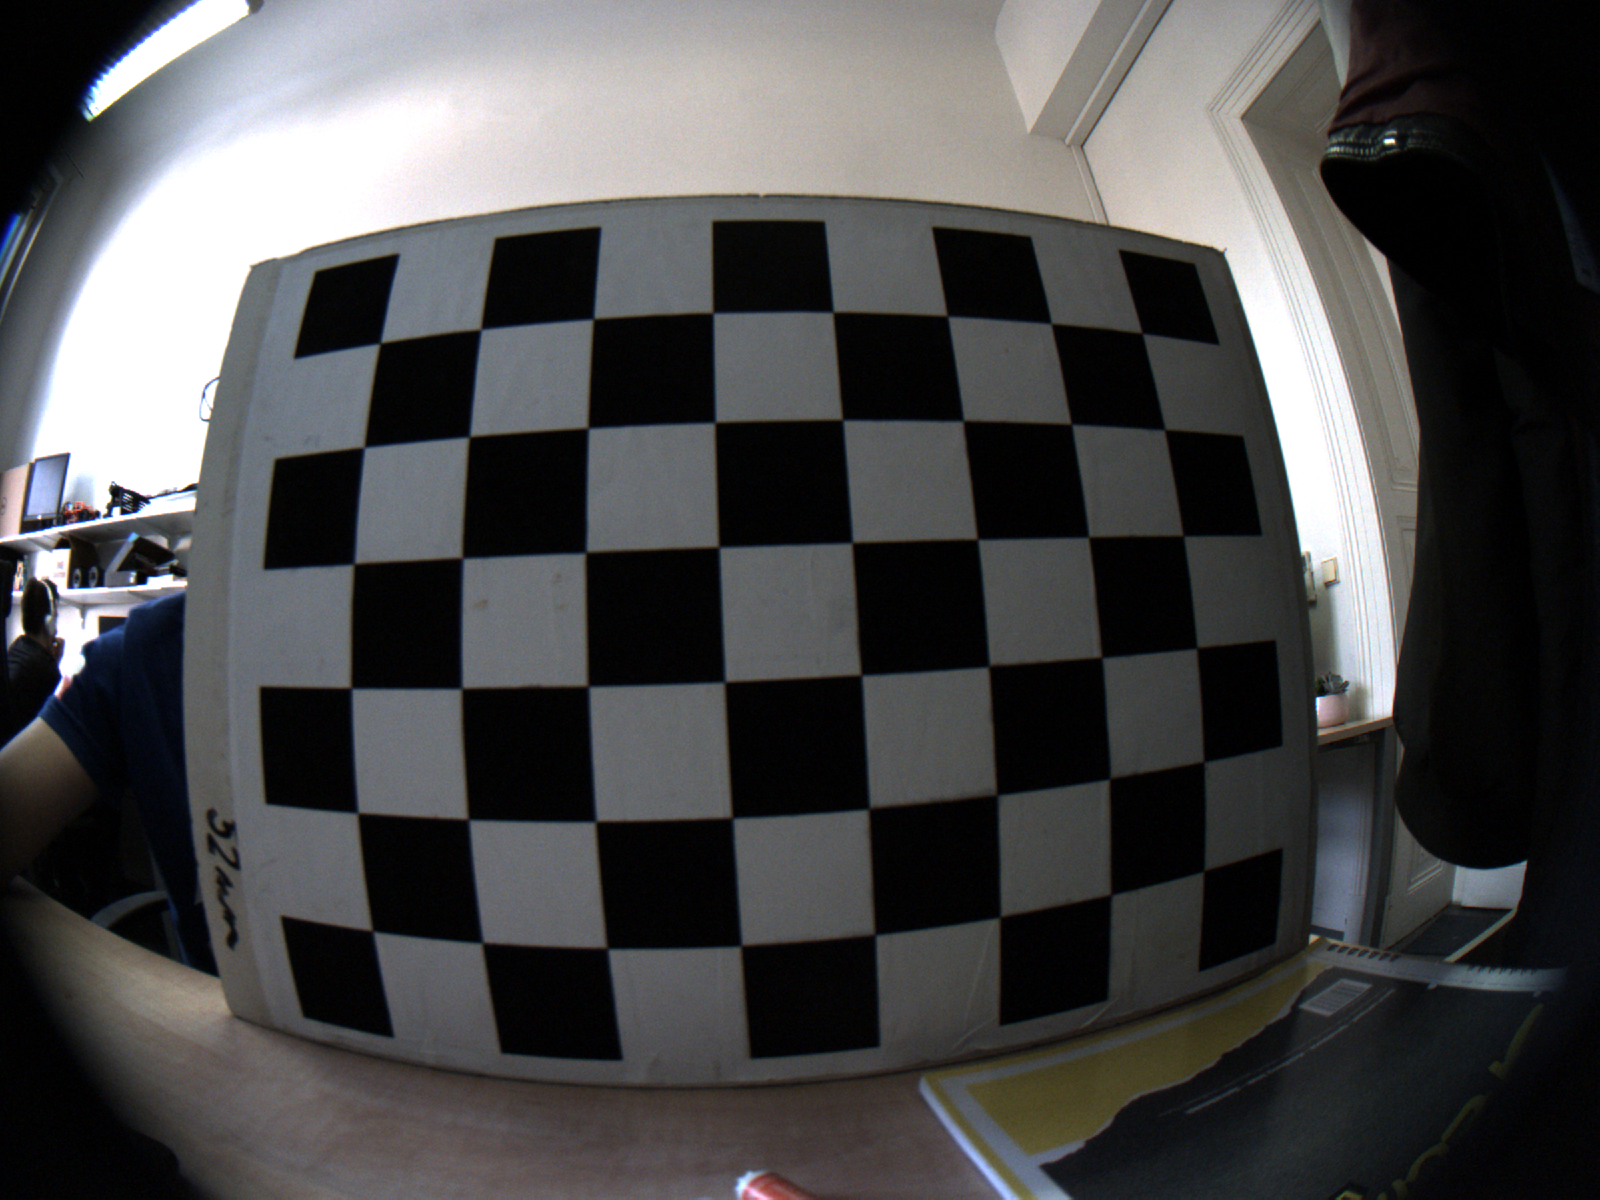
\includegraphics[width=\textwidth]{graphics/chessboard_img.png}
      \caption{Original image with radial distortion.}
      \label{fig:chb1}
    \end{subfigure}
    \hfill
    \begin{subfigure}[b]{0.45\textwidth}
      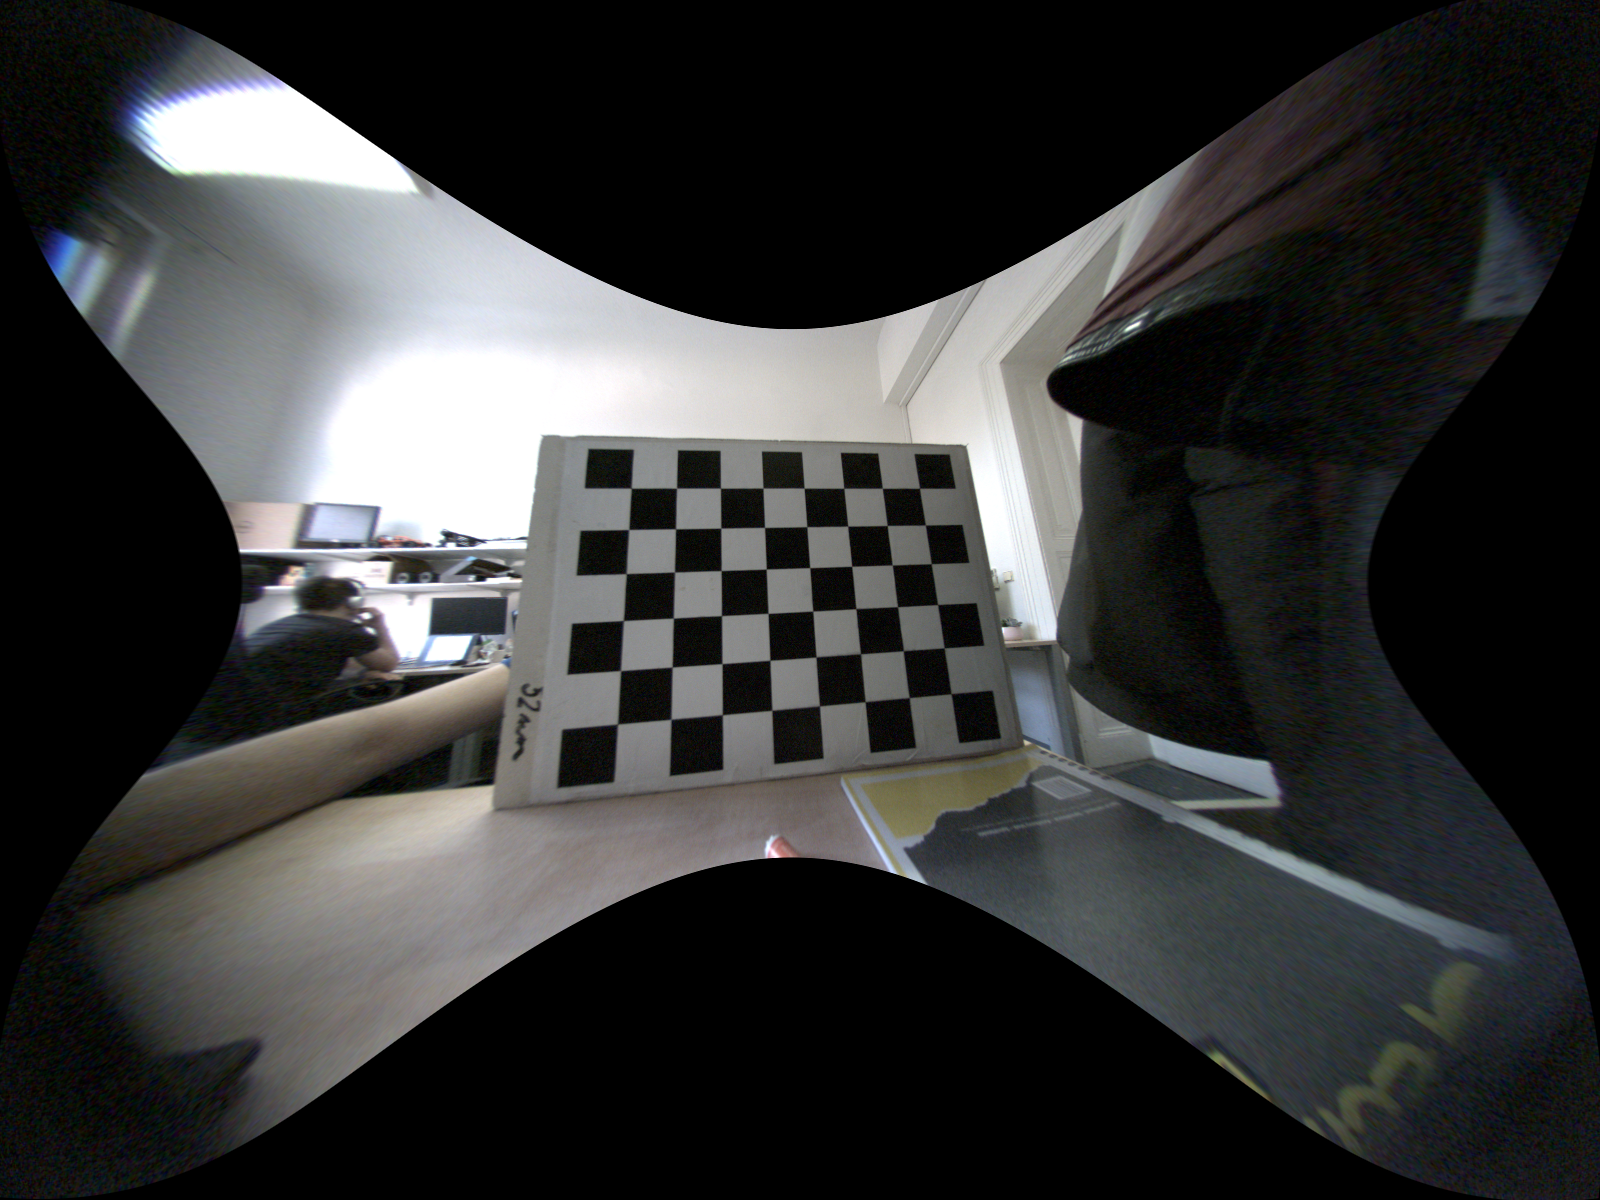
\includegraphics[width=\textwidth]{graphics/chessboard_img_rect.png}
      \caption{Rectified image with no distortion.}
      \label{fig:chb2}
    \end{subfigure}
    \caption{Camera image before and after the calibration}
    \label{fig:chb}
\end{figure}

Camera calibration - or \textit{Camera resection} process of computing the camera calibration matrix $K$ (\autoref{eq:kmat}).
Usually, it is done with some pattern with predefine parameters, as a chessboard or more advanced boards (ArUco and ChArUco\footnote{\href{https://docs.opencv.org/4.x/df/d4a/tutorial_charuco_detection.html}{Opencv ChArUco and ArUco boards}}).

Camera calibration is necessary for geometry correction (\autoref{fig:chb}), so as a result parallel lines in 3D are parallel on the image after the rectification and image unwraped and projected on a plane.

In a real world lenses has also some distortion (\autoref{fig:chb1}) so to fix that distortion coefficients should be calculated: radial distortion $k_1, k_2, k_3, k_4, k_5, k_6$ and tangential distortion $p_1, p_2$.

From the \autoref{eq:projection}:
\begin{equation}
    \label{eq:dist_start}
    \lambda \begin{bmatrix} 
        u \\ v \\ 1 \end{bmatrix} = K [R | \vec{t}] \begin{bmatrix} x \\ y \\ z \\ 1
    \end{bmatrix}
\end{equation}
\begin{equation}
    \begin{bmatrix} x_c \\ y_c \\ z_c \end{bmatrix}
     = [R | \vec{t}] \begin{bmatrix} x \\ y \\ z \\ 1
    \end{bmatrix}
\end{equation}
\begin{equation}
    u' = \frac{x_c}{z_c} \frac{1 + k_1r^2 + k_2r^4 + k_3r^6}{1 + k_4r^2 + k_5r^4 + k_6r^6} + p_1(r + 2x') + 2p_2\frac{x_c y_c}{z^2_c}
\end{equation}
\begin{equation}
    v' = \frac{y_c}{z_c} \frac{1 + k_1r^2 + k_2r^4 + k_3r^6}{1 + k_4r^2 + k_5r^4 + k_6r^6} + 2p_1(\frac{x_c y_c}{z_c^2}) + p_2(r + 2y')
\end{equation}
where $x' = (\frac{x_c}{z_c})^2$; $y' = (\frac{y_c}{z_c})^2$; $r = x' + y'$. Then undistorted point will be
\begin{equation}
    \label{eq:dist_end}
    \begin{bmatrix} u \\ v \\ 1 \end{bmatrix} = K \begin{bmatrix} u' \\ v' \\ 1 \end{bmatrix}
\end{equation}

Considering \autoref{eq:kmat}, image of a point $X$ seen through the calibrated camera with projection matrix $P$ will look as in \autoref{eq:dist_start} - \autoref{eq:dist_end}.

\subsection{Stereopair calibration}

Stereopair calibration is a process of estimation the essential matrix $E$ for a camera pair, that also can be computed from a relative rotation matrix $R_{21}$ and a relative translation vector $\vec{t_{21}}$ of a camera pair. One of approaches is to fix one camera  pose as world coordinate frame origin $C_1 = (0, 0, 0)^T$ and compute a pose of a second camera with respect to the first one. This can be done with a PnP (Perspective-n-Point) problem solver - estimation of a calibrated camera pose given a set of $n$ 3D points in a world coordinate frame. Minimal required $n=3$. 

Another possible approach is given an initial guess of a cameras poses and two sets of 3D points from both cameras fix the error by minimisation of the transformation between that point sets. This approach is described in \cite{Umeyama1991}, "Least-squares estimation of transformation parameters between two point patterns" - estimateion of needed $R$ and $\vec{t}$.